% !TEX root = main.tex

\section{Introduction}

Symbolic execution is a powerful program analysis technique first introduced in the mid 70's in the context of software testing to check if a certain property $\phi$ is violated by a program~\cite{K-ICRS75,SELECT-ICRS75,K-CACM76,H-TSE77}.
\mynote{
[D] added two references from '75, check what they cite
%IF: are references appropriate? Should we give more credits? It seems several groups introduced independently this technique
}
For instance, $\phi$ could be: ``no division by zero is ever performed'', ``no {\tt NULL} pointer is ever dereferenced'', or ``no backdoor exists that can bypass authentication''. While in general there is no automated way to decide some properties, e.g., ``does a program always terminate?'', often decidable approximations exist that can prove useful in practice in a variety of applications including mission-critical and security applications, e.g., ``does a program always terminate within a certain amount of time?''

A concrete execution can only underapproximate the analysis of a property under a given workload by exploring a single control flow path. In contrast, symbolic execution can simultaneously explore multiple paths that a program could take under different inputs. This paves the road to sound analyses that can yield strong guarantees on the checked property. Symbolic execution may answer useful questions on concrete programs like: ``does function {\tt foo(x)} always return a positive value for any possible value of {\tt x}?'' The key idea behind symbolic execution is to allow a program to take on ``symbolic'' -- rather than concrete -- input values. Execution is performed by an {\em abstract machine}, which maintains for each explored control flow path: (i) a first-order Boolean {\em formula} that describes the conditions satisfied by the branches taken on that path, and (ii) a {\em symbolic store} that maps variables to symbolic expressions. Branch execution updates the formula, while assignments update the symbolic store. A model checker, typically based on a SMT solver\mynote{add citation}, is used to verify if there are any violations of property $\phi$ along each explored path and if the path itself is realizable, i.e., its formula is satisfied by some assignment of concrete values to the program's symbolic arguments.

%Variables and control flow paths are associated with expressions and constraints in terms of those symbols during a symbolic execution of the program, and constraints are eventually solved via SMT (satisfiability modulo theories) solvers.

In this article, we survey the main aspects of symbolic execution and discuss its extensive usage in testing and computer security applications\mynote{IF: want focus only on security?}, where software vulnerabilities can be found by symbolically executing programs at the level of either source or binary code. We start with a simple example that highlights many of the fundamental issues that we address in this article.

\subsection{Warm-up example}
\label{symbolic-execution-example}

We consider the C example of Figure~\ref{fig:example-1}, analyzing for which inputs the  {\tt assert} at line 8 of function \texttt{foobar} fails. Each input parameter {\tt a} and {\tt b} can take $2^{32}$ distinct integer values. A possible approach is to concretely execute the function on randomly generated inputs.
%Techniques such as random testing could generate bottomless input tests for this function. 
However, it is unlikely that exactly the assert-failing inputs would be randomly picked up\mynote{Fuzzing?}. 
Symbolic execution overcomes these limitations by evaluating a piece of code using {\em symbols}, instead of concrete values, for its inputs. This makes it possible to reason on {\em classes of input values}, instead of single input instances. 

\begin{figure}[t]
\begin{lstlisting}[basicstyle=\ttfamily\small]
              1.  void foobar(int a, int b) {
              2.     int x = 1, y = 0;
              3.     if (a != 0) {
              4.        y = 3+x;
              5.        if (b == 0)
              6.           x = 2*(a+b);
              7.     }
              8.     assert (x-y != 0);
              9.  }
\end{lstlisting}
\caption{Simple C function used in the warm-up example.}
\label{fig:example-1}
\end{figure}

In more detail, every value that cannot be statically determined, such as an actual parameter of a function or the result of a system call that reads data from a stream, is represented by a symbol $\alpha_i$. The analysis is carried out by a {\em symbolic execution engine}, which explores several computation paths simultaneously and checks the desired property along the way. 

To discuss our example, we first briefly recall how a generic symbolic execution engine works. At any time, the engine maintains a state $(stmt,~\sigma,~\pi)$ where:

\begin{itemize}

\item $stmt$ is the next statement to evaluate. For the time being, we assume that $stmt$ can be an assignment, a conditional branch, or a jump (a discussion of more complex constructs such as function calls will be provided in later sections).

\item $\sigma$ is a {\em symbolic store} that associates program variables with expressions over concrete and symbolic values $\alpha_i$.

\item $\pi$ is {\em path constraint}, i.e., a formula that expresses a set of assumptions on the symbols $\alpha_i$ due to branches taken in the execution to reach $stmt$. At the beginning of the analysis, the path constraint is the constant $true$ formula.

\end{itemize}

\noindent Depending on $stmt$, the symbolic engine changes the state as follows:

\begin{itemize}
  \item The evaluation of an assignment $x=e$ changes the symbolic store $\sigma$ by associating $x$ with a new symbolic expression $e_s$. We denote this association with $x\mapsto e_s$, where $e_s$ is obtained by evaluating $e$ in the context of the current execution state and  can be any expression involving unary or binary operators over symbols and constant values over a concrete domain.
  
%   $\alpha_i = e$: when an expression $e$ is assigned to a symbol $\alpha_i$, $pc$ is extended by adding a constraint on $\alpha_i$:
%    \[ pc \gets pc \wedge \alpha_i = e\]
%  where $e$ can be any expression, involving unary or binary operators, over symbols and constants.

  \item The evaluation of a conditional branch ${\tt if}~e~{\tt then}~s_{true}~{\tt else}~s_{false}$ affects the path constraint $\pi$. Namely, the symbolic execution is forked by creating two execution states with path constraints $\pi_{true}$ and $\pi_{false}$, respectively, corresponding to the two {\tt if} branches: $\pi_{true}=\pi \wedge e_s$ and $\pi_{false}=\pi \wedge \neg e_s$, where $e_s$ is a symbolic expression obtained by evaluating $e$. 
%        \[ (s_{true}, pc_{true}) \text{ where } pc_{true} = pc \wedge e \]
%        \[ (s_{false}, pc_{false}) \text{ where } pc_{false} = pc \wedge \neg e \]
    Symbolic execution proceeds on both states in parallel.

  \item The evaluation of a jump {\tt goto} $s$ updates the execution state by advancing the symbolic execution to statement $s$. 
\end{itemize}

%\subsection{Example}
%\label{symbolic-execution-example}

%\begin{figure}[t]
%  \centering
%  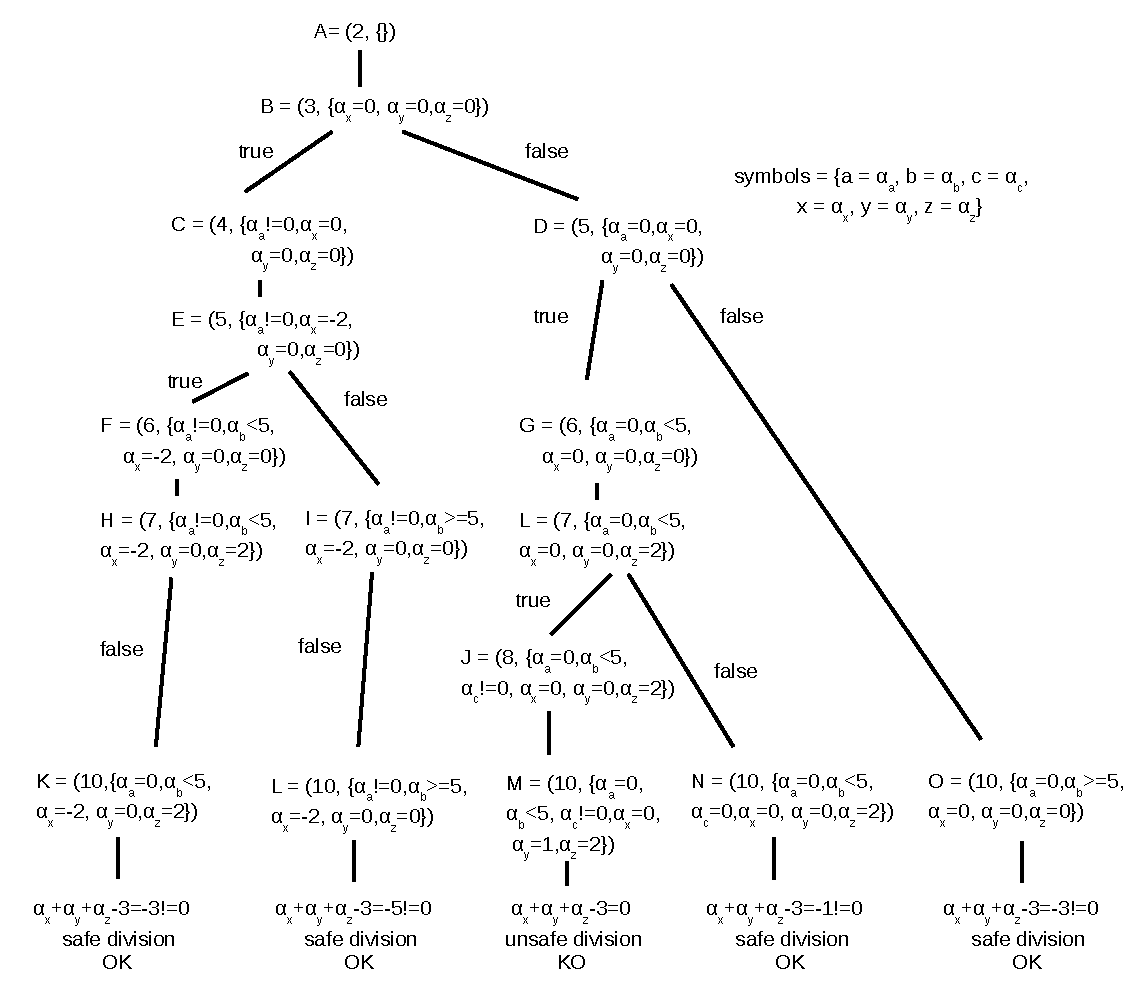
\includegraphics[width=1.0\columnwidth]{images/example} 
%  \caption{Symbolic execution tree of the function {\tt foobar}. Each execution state is labeled with an alphabet letter. Side effects on execution states are highlighted in gray. Leaves are evaluated against division by zero error. For the sake of presentation the conjunction of constraints is shown as a list of constraints. }
%  \label{fig:example-symbolic-execution}
%\end{figure}

\begin{figure}[t]
  \centering
  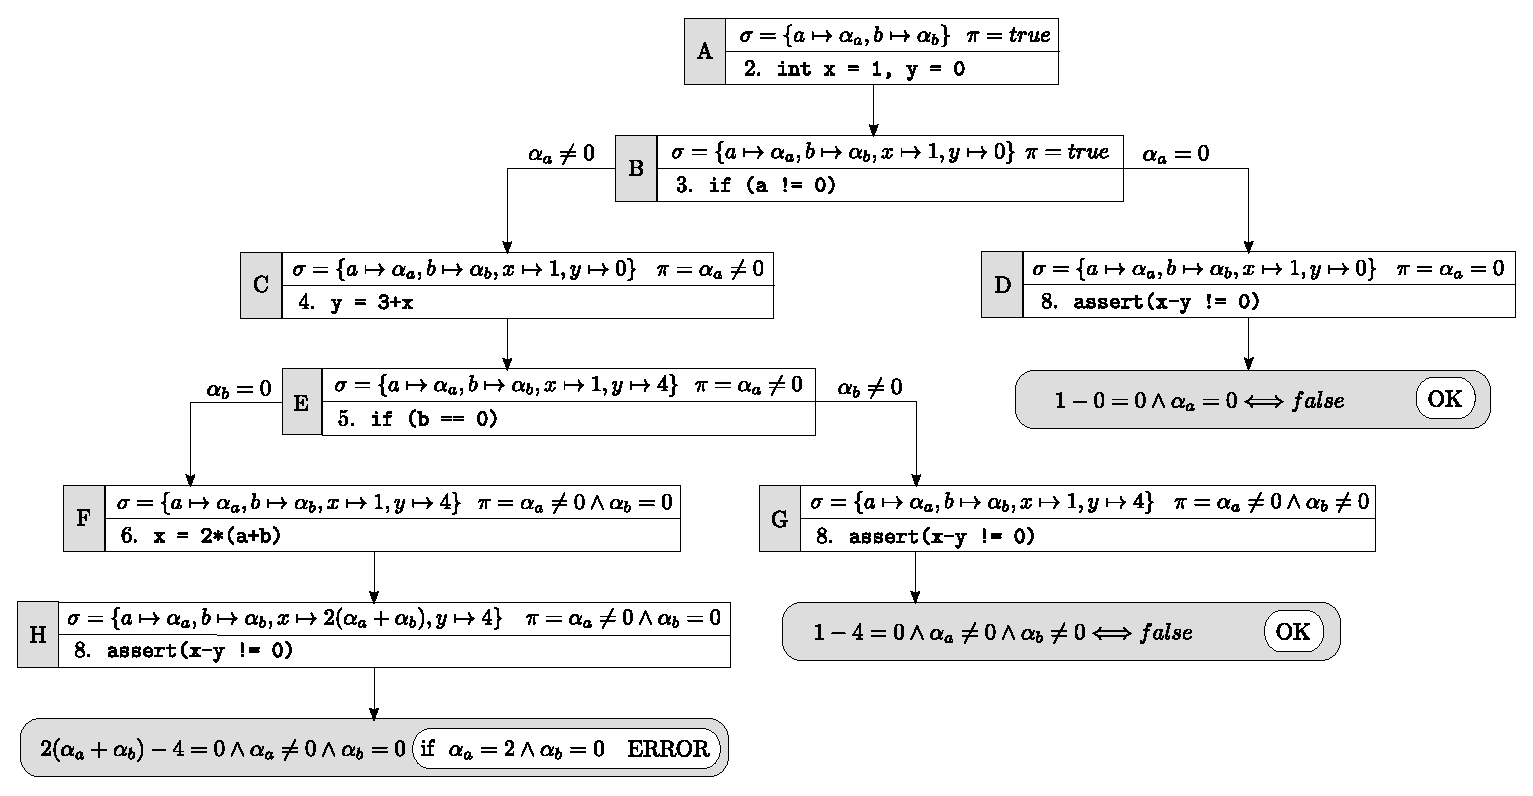
\includegraphics[width=1.0\columnwidth]{images/execution-tree.eps} 
  \caption{Symbolic execution tree of function {\tt foobar} given in Figure~\ref{fig:example-1}. Each execution state, labeled with an upper case letter, shows statement, symbolic store $\sigma$, and path constraint $\pi$. Leaves are evaluated against the condition in the {\tt assert} statement. }
%For the sake of presentation the conjunction of constraints is shown as a list of constraints. }
  \label{fig:example-symbolic-execution}
\end{figure}

\noindent A symbolic execution of function {\tt foobar} is shown in Figure~\ref{fig:example-symbolic-execution}. Initially (execution state $A$) the path constraint is {\tt true} and input arguments {\tt a} and {\tt b} are associated with symbolic values. 
After initializing local variables {\tt x} and {\tt y} at line 2, the symbolic store is updated by associating {\tt x} and {\tt y} with concrete values 1 and 0, respectively (execution state $B$). Line 3 contains a conditional branch and the execution is forked: depending on the branch taken, a different statement is evaluated next and different assumptions are made on symbol $\alpha_a$ (execution states $C$ and $D$, respectively). In the branch where $\alpha_a\neq 0$, variable {\tt y} is assigned with ${\tt x}+3$, obtaining $y\mapsto 4$ in state $E$ because $x\mapsto 1$ in state $C$. In general, arithmetic expression evaluation simply manipulates the symbolic values.
After expanding every execution state until the {\tt assert} at line 8 is reached on all branches, we can check which input values for parameters {\tt a} and {\tt b} can make the {\tt assert} fail. By analyzing execution states $\{D,G,H\}$, we can conclude that only $H$ can make {\tt x-y = 0} true. The path constraint set for $H$ at this point implicitly defines the set of inputs that are unsafe for {\tt foobar}. 
In particular, any input values such that:
 \[ 2(\alpha_a+\alpha_b)-4 = 0 \wedge \alpha_a \neq 0 \wedge \alpha_b = 0 \]
will make {\tt assert} fail. An instance of unsafe input parameters can be eventually determined by invoking a model checker to solves the path constraints, which in this example would yield $a = 2$ and $b = 0$. 

%Notice\mynote{Say earlier?} that a constraint solver is also needed when evaluating the satisfiability of branch conditions.

\subsection{Challenges in Symbolic Execution}
\label{example-discussion}

As shown in Section~\ref{symbolic-execution-example}, symbolic execution can identify {\em all} possible unsafe inputs that make the {\tt assert} fail. This is achieved through an exhaustive exploration of the possible execution states. From a theoretical perspective, symbolic execution provides a {\em sound} and {\em complete} methodology for any decidable analysis. Soundness prevents false negatives, i.e., all possible unsafe inputs are guaranteed to be found, while completeness prevents false positives, i.e.,  input values deemed as unsafe are actually unsafe. 

Challenges that symbolic execution has to face when processing real-world code can be significantly more complex than those illustrated in our warm-up example. Several observations and questions naturally arise:

\begin{itemize}

\item \noindent {\em Objects}: how does the symbolic engine handle arrays or other complex objects?
Any arbitrarily complex object can be regarded as an array of bytes and each byte associated with a distinct symbol. However, when possible, exploiting structural properties of the data may be more convenient: for instance, relational bounds on the class fields in object-oriented languages could be used for refining the search performed by symbolic execution.
\vspace{1mm}

  \item {\em Loops}: how does the symbolic engine handle loops?
%A loop\mynote{IF: rimuoverei la prima frase, perche' va detto?} can be encoded using conditional branches and {\tt goto} statements, which is typical  when compiling high-level languages to an intermediate representation or native code. 
Choosing the number of loop iterations to analyze is critical for the symbolic engine, especially when this number cannot be determined in advance (since, e.g., depends on an input parameter). The naive approach of unrolling iterations for every valid bound would result in a prohibitively large number of states. Typical solutions are to compute an underapproximation of the analysis by limiting the number of iterations to $k$, thus trading speed for soundness. Another approach is to infer loop invariants through static analysis  and use them to merge equivalent states (\mynote{Recuperare citazione}e.g., when differences are not observable outside the loop body).
\vspace{1mm}

\iffalse
  \item {\em Subroutines and recursion}: how does the symbolic engine handle subroutines and recursive calls?
In order to support subroutines, the execution state is typically provided with an execution stack. Consider the following recursive example:
    \begin{lstlisting}[basicstyle=\ttfamily\small]
    1.  int fac(int n) {
    2.    if (n <= 1) return 1;
    3.    return n*fac(n - 1);
    3.  }
    \end{lstlisting}
Note that each distinct value of {\tt n} leads to a distinct control flow path. Since {\tt n} can assume up to  $2^{31} - 1$ positive values, a symbolic engine would create as many execution states to cover all the possible paths.
%This code can easily lead to a very large number of states: a new state would be indeed created each time the branch at line 2 is not taken. Since variable {\tt n} can assume up to  $2^{31} - 1$ positive values, the symbolic engine would create as many execution states to cover all the possible paths.
 %Indeed, the number of executions states is related to the number of times that the conditional branch on line 2 is not taken. 
 \vspace{1mm}
 \fi

  \item {\em Environment}: how does the symbolic engine handle interaction with the environment?
  Real-world applications constantly interact with the environment (e.g., with the file system or the network) through libraries and system calls. These interactions may cause side-effects
(such as the creation of a file) that could later affect the execution and must be thus taken into account. Evaluating any possible interaction outcome is generally unfeasible: it could generate a large number of execution states, of which only a small number can actually happen in a non-symbolic scenario. A typical strategy is to consider popular library and system routines and to create models that can help the symbolic engine analyze only significant outcomes.
\vspace{1mm}

  \item {\em State space explosion, path selection}: how does symbolic execution deal with path explosion?
  A relatively simple code such as function {\tt foobar}, which is composed by less 12 lines of code, has generated 16 execution states, where $5$ out of $16$ are independent\mynote{Independent?} and must be checked to determine possible unsafe input values. Although this could seem a reasonable number of states, language constructs such as loops may contribute to increase the number of states exponentially. For this reason, it is unlikely that a symbolic execution engine is able to exhaustively explore all the possible execution states within a reasonable amount of time. In practice, heuristics are used to guide exploration and prioritize certain states first (e.g., to maximize code coverage), hoping this would lead to interesting discoveries. Also, a symbolic execution engine should implement efficient mechanism for evaluating multiple execution states in parallel without running out of resources.
  %In practice, several heuristics must be exploited to prioritize evaluation of some states, hoping to still be able to spot interesting things. Moreover, the symbolic execution engine should include efficient mechanism for efficiently evaluating in parallel different execution states without running out of computational resources.
\vspace{1mm}

  \item {\em Constraint solver}: what can a constraint solver do in practice?
  %{\em What is a constraint solver in practice}? \\
 Constraint solvers suffer from a number of limitations. Typically, they can handle complex constraints in a reasonable amount of time only if they are made of linear expressions over their constituents. Symbolic execution engines typically implement a number of optimizations to make queries as much {\em solver-friendly} as possible, for instance by splitting queries in independent components to process separately or by performing algebraic simplifications.
\vspace{1mm}

  \item {\em Binary code}: what are the disadvantages of symbolically executing binary code?
  The example presented in Section~\ref{symbolic-execution-example} is written in C. This does not imply that symbolic execution cannot be performed directly on binary code, which in several scenarios is the only available representation of a program. However, having the source code of an application makes symbolic execution significantly easier, as it can exploit high-level properties (e.g., object shapes) that can be inferred by statically analyzing the source code.
  %(e.g., the maximum size of a buffer or the number of iterations for a loop).
   
\end{itemize}
%Depending on the specific application context of symbolic execution
Depending on the specific context in which symbolic execution is used, different choices and assumptions are made to address the questions highlighted above. Although they typically affect soundness or completeness, in several scenarios a partial exploration of the space of possible execution states is typically sufficient to reach the goal\mynote{Better example?} (e.g., identify a crashing input for an application) with a limited time budget.

%different choices and assumptions are made to address the above questions. Although soundness and completeness of symbolic execution may be negatively affected by these choices, there are several application scenarios where a partial exploration of the possible execution states is sufficient for reaching the ultimate goal (e.g., identify a single input that crashes an application).

\subsection{Organization of the Article}

The remainder of this article is organized as follows. In section .

%\vspace{2cm}
%\subsection{Removed stuff}
%
%\paragraph{Black-box approach versus white-box approach}
%
%Discussion\mynote{IF: do we really need this?} of black-box approach and white-box approach. Symbolic execution is a white-box technique. Black-box approaches can be very fast but not always effective. White-box approaches can be very effective but are typically slower than black-box techniques. An in-depth discussion of this aspect will be done when we will discuss~\cite{DRILLER-NDSS16}.
%
%\begin{figure}[H]
%  \vspace{-3mm}
%  \centering
%  \begin{subfigure}{.5\textwidth}
%    \centering
%    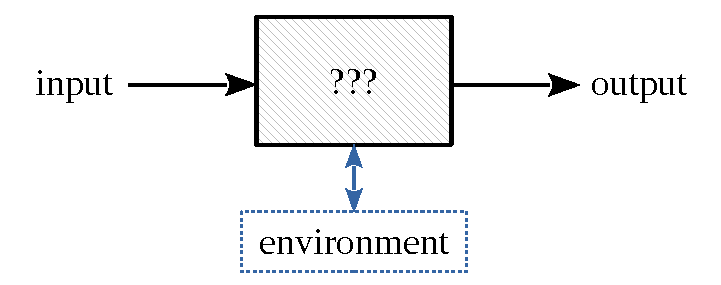
\includegraphics[width=0.9\linewidth]{images/blackbox} 
%    \caption{Black-box approach}
%    %\label{fig:sub1}
%  \end{subfigure}%
%  \begin{subfigure}{.5\textwidth}
%    \centering
%    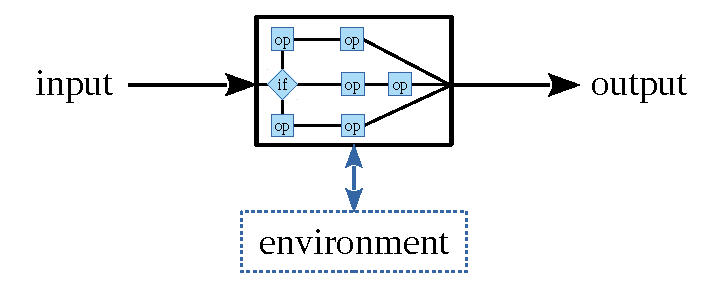
\includegraphics[width=0.9\linewidth]{images/whitebox} 
%    \caption{White-box approach}
%    %\label{fig:sub2}
%  \end{subfigure}
%  %\label{fig:example-symbolic-execution}
%  \vspace{-3mm}
%\end{figure}
%
%\paragraph{Taken from old Overview}
%
%Symbolic execution has been originally introduced in~\cite{K-CACM76} and~\cite{H-TSE77}. A good introduction to symbolic execution is presented in~\cite{KLEE-OSDI08}.\mynote{Extend this paragraph}
%%(while~\cite{EXE-CCS06} is a previous effort of the same authors).
%\cite{SAGE-NDSS08} is one successful story of symbolic execution. \cite{SAB-SP10} presents a neat formalization of symbolic execution and of taint analysis as well.
%
